\documentclass{homework}
% \usepackage{graphicx} % Required for inserting images
\usepackage{amsmath}
\usepackage{gensymb}
\usepackage{subfig}
\usepackage{float}

\class{APPM 5560}
\title{Homework 6}
\author{Sean Jennings}
\date{March 13, 2024}

\begin{document}
\maketitle

\section{Problem 1}
The system can be described by a 2-state Markov chain, with
State 1 being a sunny day and state 2 cloudy. The
transition matrix given by:
\begin{equation*}
    p = \mat{
        1 - a & a \\
        b & 1 - b
    }
\end{equation*}
where $a = 1/4$ is the probability of going from a sunny day to 
a cloudy day, and $b = 2/3$ is the probability of going from a cloudy
to sunny.

From previous homework, we showed that the stationary distribution for
such a markov chain is given by:
\begin{align*}
    \pi &= \mat{\frac{b}{a + b} & \frac{a}{a+b}} \\
        &= \mat{\frac{2/3}{11/12} & \frac{1/4}{11/12}} \\
        &= \mat{8/11 & 3/11}
\end{align*}
The fraction of sunny days is then given by first entry of the stationary
distribution $\pi(1) = 8/11$.


\section{Problem 2}
\begin{letterenum}
\item Figure \ref{fig:mc} shows the markov chain for the disease progression.
The probability transition matrix (in order E,M,S,D,H) is given by
\begin{equation*}
    p = \mat{
        0.7 & 0.1 & 0 & 0 & 0.2 \\
        0 & 0.3 & 0.3 & 0.2 & 0.2 \\
        0 & 0 & 0.4 & 0.3 & 0.3 \\
        0 & 0 & 0 & 1 & 0 \\
        0 & 0 & 0 & 0 & 1
    }
\end{equation*}

\begin{center}
    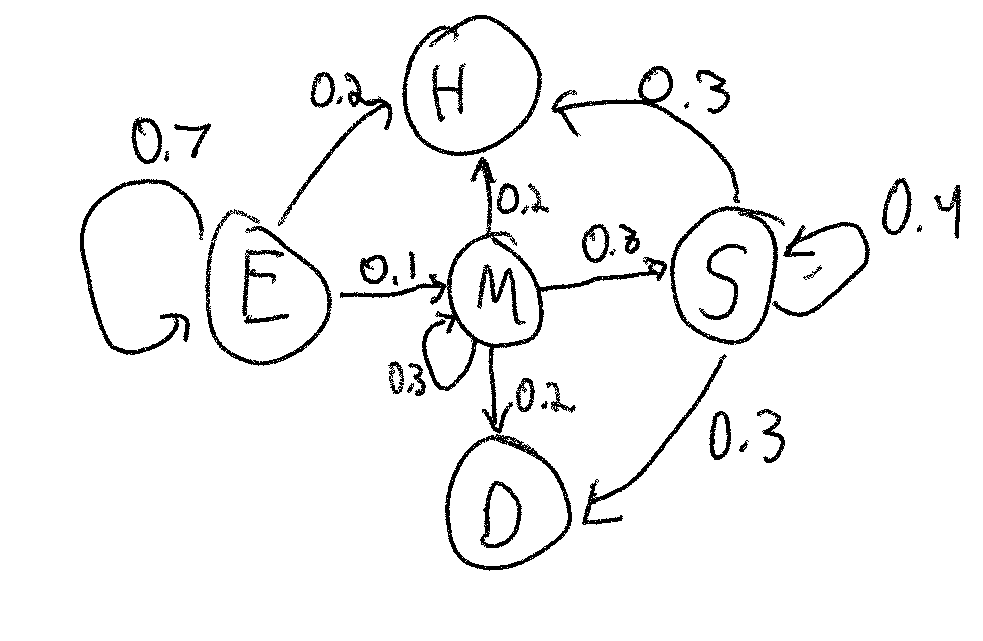
\includegraphics[width=0.8\linewidth]{Images/markov_chain.png}
    \captionof{figure}{Markov Chain for Disease States}
    \label{fig:mc}
\end{center}

\item Let $N_i$ be the number of steps until a person starting in state $i$
either dies or becomes healthy. Then, by the total expectation theorem,
the expected number of days for someone in state S is:
\begin{align*}
    N_S &= {\bf P}(\text{dies or become healthy}) 1 +
             {\bf P}(\text{remains in }S) (N_S + 1) \\
        &= 1 + 0.4 N_S \\
        &= 1 / (1 - 0.4) = 5/3
\end{align*}
Similarly, for a mildly ill person:'
\begin{align*}
    N_M &= 0.3 (N_M + 1) + 0.3 ( N_S + 1) + 0.4 \\
        &= \frac{0.3 N_S + 1}{1 - 0.3} = 15/7
\end{align*}
and finally for an exposed person:
\begin{align*}
    N_E &= 0.1 (N_M + 1) + 0.3 (N_S + 1) + 0.4 \\
        &= \frac{0.1 N_M + 1}{1 - 0.7} = 85/21 \approx 4.047
\end{align*}
So the expected number of days until an exposed person either dies or becomes
healthy is slightly greater than 4 days.

\item Let $\rho_{ij}$ be the probability that starting at state $i$, the state
reaches state $j$ for some finite time. Then, the probability an exposed person
becomes healthy is $\rho_{EH}$. Starting with a severe disease state, we have

\begin{align*}
    \rho_{SH} = 0.3 + 0.4 \rho_{SH} = \frac{0.3}{1 - 0.4} = 3/7
\end{align*}
From $M$, we have
\begin{align*}
    \rho_{MH} &= 0.3 \rho_{MH} + 0.3 \rho_{SH} + 0.2 \\
        &= \frac{0.3 (3/7) + 0.2}{1 - 0.3} \\
        &= \frac{23}{49}
\end{align*}

And finally, for an exposed person:
\begin{align*}
    \rho_{EH} &= 0.2 + 0.7 \rho_{EH} + 0.1 \rho_{MH} \\
        &= \frac{0.2 + 0.1 (23/49)}{1 - 0.7} \\
        &\approx 0.823.
\end{align*}
So there is about a 82.3\% chance an exposed person will recover.

\end{letterenum}
\section{Problem 3}

\begin{letterenum}
\item From HW3, the probability transition matrix is given by:
\begin{equation*}
    \mat{
        0 & 1 & 0 & 0 & 0 \\
        1/3 & state0 & 2/3 & 0 & 0 \\
        0 & 1/2 & 0 & 1/2 & 0 \\
        0 & 0 & 2/3 & 0 & 1/3 \\
        0 & 0 & 0 & 1 & 0 \\
    }
\end{equation*}
Figure \ref{fig:grid-mc} shows the chain.

\begin{center}
    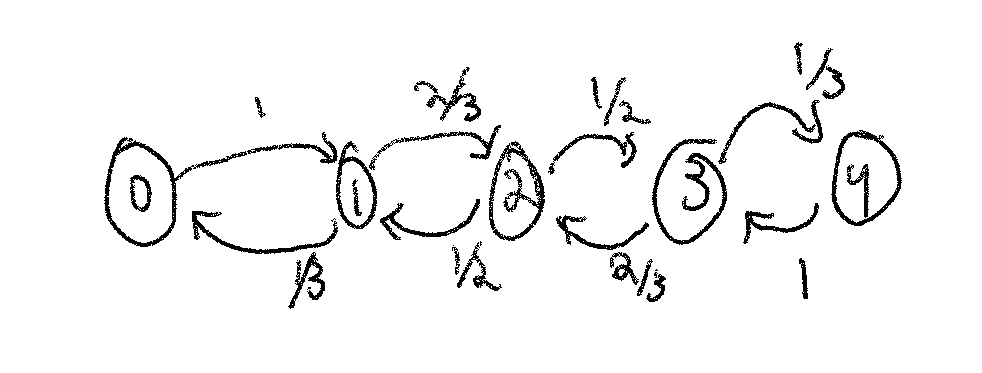
\includegraphics[width=0.8\linewidth]{Images/grid_chain.png}
    \captionof{figure}{Markov chain for sum of x and y coordinates}
    \label{fig:grid-mc}
\end{center}

We check the detailed balance condition to find a stationary distribution:
\begin{align*}
    \pi(1) &= \frac{1}{1/3} \pi(0) = 3 \pi(0) \\
    \pi(2) &= \frac{2/3}{1/2}\pi(1) = 4/3 \pi(1) = 4 \pi(0) \\
    \pi(3) &= \frac{1/2}{2/3}\pi(2) = 3/4 \pi(1) = 3 \pi(0) \\
    \pi(4) &= \frac{1/3}{1}\pi(3) = \pi(0)
\end{align*}
So the stationary distribution is given by:
\begin{equation*}
    \pi = \pi(0) \mat{1 & 3 & 4 & 3 & 1}.
\end{equation*}
By normalization, we find $\pi(0) = 1/12$ so that the stationary
distribution is:
\begin{equation*}
    \pi = \mat{1/12 & 1/4 & 1/3 & 1/4 & 1/12}.
\end{equation*}
This distribution is unique since the markov chain is finite and irreducible.

\item For each $i\in S$, we have:
\begin{align*}
    p(i, i) = 0 &\qquad p^2(i, i) > 0 \\
    p^3(i, i) = 0 &\qquad p^4(i, i) > 0 
\end{align*}
and so on for odd and even powers of $p$. The chain therefore has period 2
and is not aperiodic. Therefore, it will not converge to the stationary
distribution.

\item Figure \ref{fig:q_100} shows the plot of $q_{100}(i)$ and $\pi(i)$
vs. $i$, starting from
\begin{equation*}
    q_0 = \mat{0 & 1 & 0 & 0 & 0}
\end{equation*}
(in other words, $X_0 = 1$ with probability 1). We see that, as predicted
in the previous subproblem, the state does not converge to the stationary
distribution. For even $n$, the distribution $q_n$ has only states 1 and 3
with nonzero probability. For odd $n$, the distribution $q_n$ has 0, 2, and 4
with nonzero probability. It alternates between such distributions with period
2.

\begin{center}
    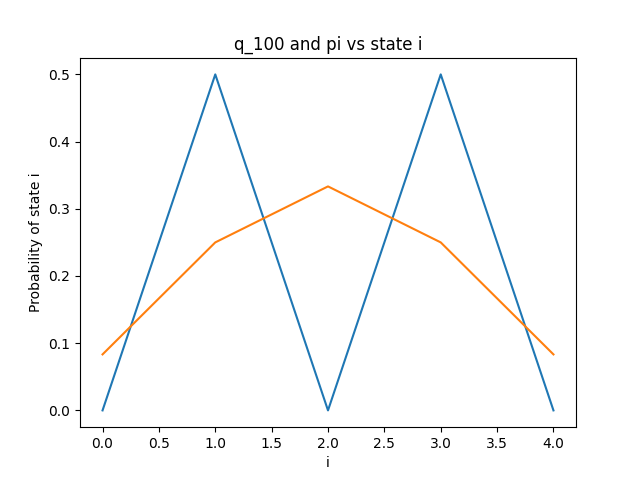
\includegraphics[width=0.8\linewidth]{Images/q_100.png}
    \captionof{figure}{Plot of q\_100 vs stationary distribution}
    \label{fig:q_100}
\end{center}

\end{letterenum}

\section{Problem 4}
In the long run, the fraction of the population living in each area is
equivalent to the stationary distribution. We use the numerical eigenvalue-based
routine from the previous HW and find the stationary distribution to be:
\begin{equation*}
    \pi \approx \mat{0.5634 & 0.3099 & 0.1268}.
\end{equation*}
So $\sim$56\% of the population will be urban, $\sim$31\% suburban, and $\sim$13\%
rural.

\section{Problem 5}
\begin{letterenum}
\item We again use a numerical routine to find the stationary distribution:
\begin{equation*}
    \pi \approx \mat{
        0.5854 & 0.2427 & 0.0976 & 0.0244
    }
\end{equation*}

If David shaves on day $n-1$, then the state of the markov chain on day $n$
is $X_n = 1$. Therefore, the long-run fraction of time that David shaves is
the probability that he shaved on a day $n-1$ for some large $n$.
This is equivalent to the entry in the stationary distribution corresponding
to state 1: $\pi(1) = 0.5854$.

\item The stationary distribution does not satisfy detailed balance.
For example, the state can go from state 3 to state 4, but not the opposite
direction. Therefore, we have $\pi(3) > 0$, $p(3, 4) > 0$ and $p(4, 3) = 0$,
which implies that
\begin{equation*}
    \pi(3) p(3,4) \neq 0 = \pi(4) p(4,3)
\end{equation*}
    
\end{letterenum}

\section{Problem 6}

For simplicity of modulo arthmitic, we define the state space
$S = \{0, 1, \dots, 11\}$ to be 1 less than the given 1-indexed numbers.

By symmetry, the number of steps until the chain returns to its starting position
does not depend on the starting position. Therefore, let $N$ be the first nonzero
time at which the chain reaches state 0:
\begin{equation*}
    N = \min_{n>0} \{n: X_n = 0\}
\end{equation*}

Now, we define $N_i$ to be the expected time to reach state 0, given that
we start in state $i$:
\begin{equation*}
    N_i = {\bf E}[N | X_0 = i]
\end{equation*}

The expected number of steps until $X_n$ returns to its original state
is therefore $N_0$.

Again, by a symmetry argument, state 1 (number 2 on clock) and state 11
(number 12) are expected to return to state 0 (number 1) in the same amount
of time. Therefore, $N_1 = N_{11}$. In general, by clockwise/counter-clockwise
symmetry, we have 
\begin{equation*}
    N_j = N_{-j \% 12} = N_{12 - j}
\end{equation*}
for each $j = 0,1, 2, \dots, 11$.

Now, using the total expectation theorem, we find the following expression
for $N_j$:
\begin{align}
    N_j &= {\bf E}[N | X_0 = j] \\
        &= p(j, j-1) {\bf E}[N | X_1 = j-1] + p(j, j+1) {\bf E}[N | X_1 = j+1]  \\
        &= 0.5 (N_{j-1} + 1) + 0.5 (N_{j+1} + 1) \\
        &= 0.5 (N_{j-1} + N_{j+1}) + 1 \label{eq:diff-eq}
\end{align}
which holds for $j=2, 3\dots, 6$. We note that (\ref{eq:diff-eq}) does
not hold for $j=1$ since the relation:
\begin{equation*}
    {\bf E}[N | X_1 = j] = {\bf E}[N | X_0 = j] + 1 = N_j + 1
\end{equation*}
holds only for $j>0$. On the other hand, for $j=0$,
\begin{equation*}
    {\bf E}[N | X_1 = 0] = 1 \neq N_0 + 1
\end{equation*}
since we have defined $N$ as the first {\it nonzero} $n$ which has $X_n = 0$, 

(\ref{eq:diff-eq}) defines a difference equation, for which we will
use diff-eq techniques to find an analytic solution.
We now consider boundary conditions at $j=1$ and $j=6$.
At $j=1$ (since there is 0.5 probability $X_1 = 0$ starting from $X_0 = 1$
so that $N_1=1$):
\begin{equation}
    N_1 = 0.5 \cdot 1 + 0.5 (N_2 + 1) = 0.5 N_2 + 1
    \label{eq:n1}
\end{equation}

At $j=6$, by symmetry we have $N_5=N_7$ so that:
\begin{equation}
    N_6 = 0.5(N_5 + 1) + 0.5 (N_7 + 1) = N_5 + 1
    \label{eq:n6}
\end{equation}


Since the difference equation (\ref{eq:diff-eq})
is inhomogenous, we assume that $N_j$ takes the form
\begin{equation*}
    N_j = N_j^H + N_j^P
\end{equation*}
where $N_j^H$ is the homogenous solution to (\ref{eq:diff-eq}) and $N_j^P$
is the particular solution.

We assume the homogenous term takes the form $N_j^H = r^j$ and substitute
into equation (\ref{eq:diff-eq}) with the inhomogenous term removed:
\begin{equation*}
    r^j = 0.5 (r^{j-1} + r^{j+1})
\end{equation*}
Rearranging terms yields

\begin{equation*}
    0.5 (r^2 - 2r + 1) = 0
\end{equation*}
which has a single root of $r=1$ with multiplicity 2. Due to the
non-unit multiplicity, we therefore
also use $N_j^H = jr^j$ as a potential solution which with $r=1$ yields
\begin{equation*}
    N_j^H = C_0 + C_1 j
\end{equation*}
where $C_0,C_1$ are coefficients which will be used to satisfy boundary conditions.

We now find an inhomogenous term $N_j^P$ which satisfies:
\begin{equation}
    N_j^P = 0.5 (N_{j-1}^P + N_{j+1}^P) + 1.
    \label{eq:inhomogenous}
\end{equation}
We guess the simplest polynomial form which is not spanned by the homogenous
solution: $N_j^P = C_P j^2$ for some constant $C_P$. Substituting into
(\ref{eq:inhomogenous}) yields
\begin{align*}
    C_Pj^2 &= 0.5 C_P \bigl( (j-1)^2 + (j+1)^2 \bigr) + 1 \\
        &= 0.5 C_P\bigl((j^2 - 2j + 1) + (j^2 + 2j + 1)\bigr) + 1 \\
        &= C_P(j^2 + 1) + 1
\end{align*}
and we see that $j^2$ terms cancel and $C_p = -1$ satisfies the relation for all $j$.

Combining homogenous and inhomogenous solutions, we have
\begin{equation}
    N_j = C_0 + C_1j - j^2
    \label{eq:full-solution-with-constants}
\end{equation}

and we can finally substitute into boundary conditions to find constants $C_0$
and $C_1$. First putting (\ref{eq:full-solution-with-constants})
into (\ref{eq:n1}), we have
\begin{equation*}
    C_0 + C_1 - 1 = 0.5 (C_0 + 2C_1 - 4) + 1.
\end{equation*}
The $C_1$ and constant terms cancel out so that $C_0 = 0$. Now, putting
(\ref{eq:full-solution-with-constants}) into (\ref{eq:n6}), we have
\begin{equation*}
    6(C_1 - 6) = 5(C_1 - 5) + 1 \Rightarrow C_1 = 36-25+1 = 12
\end{equation*}

Thus, for $j=1,\dots,6$ we have the solution $N_j = j(12 - j)$, which
is enumerated below for ease of inspection:
\begin{align*}
    N_1 = 11 &\qquad N_4 = 32 \\
    N_2 = 20 &\qquad N_5 = 35 \\
    N_3 = 27 &\qquad N_6 = 36 \\
\end{align*}

Finally, the variable of interest $N_0$ can be found:
\begin{equation*}
    N_0 = 0.5 (N_1 + 1) + 0.5 (N_{11} + 1) = N_1 + 1 = 12
\end{equation*}
So the expected number of steps until $X_n$ returns to its starting position
is 12.

\end{document}
